When incoming energy is sufficient to run multiple consecutive tasks,
committing state after each task is wasteful. \sys mitigates this
waste by deferring the expensive commits and performing them in a
batch. In the resulting execution, several tasks are \emph{merged} into a
single virtual task---a process we call \emph{coalescing}. 
%
When $N$ tasks are coalesced, $N-1$ boundaries are crossed and some number of
pages are dirtied. The first $N-2$ executions of \transition statement skip
committing dirty pages to non-volatile memory, leaving the work of committing
pages modified by any of the $N$ tasks to the statement $N-1$.
Coalescing is likely to reduce the total number of non-volatile memory
accesses, because when coalesced tasks access the same pages of data, only the
last version of the page needs to be committed.  \textcolor{red}{maybe is possible to demonstrate with data? count number of executed non-volatile vs volatile accesses}

\textbf{Trade-off between Speed and Wasted Effort.} \sys can coalesce an
arbitrary number of consecutive tasks. However, as more tasks coalesce, their
collective commit overhead amortizes better, but the risk of wasting work also
increases. If power fails during a long sequence of coalesced tasks, execution
will restart from the last commit, i.e. the first task in the sequence, losing
the progress made by any of the coalesced tasks.  The challenge to coalescing
tasks is determining how many tasks to coalesce before committing.
%
%During execution, an executing task is either a {\em coalesced} task, which
%does not commit its state before transitioning or a {\em committing} task,
%which does commit its state before transitioning.

\textbf{Task Coalescing Strategies.} 
%
The likelihood that a task group will complete depends on the total amount of
energy consumed by all tasks in the group, i.e. the size of the dynamic task.
%
A good coalescing strategy must moderate the risk of wasted work and capitalize
on benefits of deferred commits by adapting the target size of the dynamic task
to the energy available at runtime.
%
The general structure of our strategies is to increase the target task size by
some positive delta $C_\text{up}$ after the dynamic coalesced task completes,
and decrease it by some negative delta $C_\text{down}$ upon a reboot after a
power failure.
%
The choice of $C_\text{up}$ and $C_\text{down}$, including their units, defines
the strategy and its performance.
%
For example, a naive strategy that fixes $C_\text{up}$ and $C_\text{down}$ to
``one static task``, will be very slow to react to changes in incoming energy,
since its dynamic task size can only change by the size of one (small) static
task per charge-discharge cycle.
%
Working from these observations, we propose and evaluate two coalescing
strategies for \sys: \textbf{History-aware Coalescing (HC)} and
\textbf{Task-size- and History-aware Coalescing (TSHC)}.

\textcolor{red}{Replace the following with definition of all coalescing strategies}

%\begin{enumerate}
%	\item \textbf{Interrupt History Coalescing (HDC):} when more tasks are coalesced without power interrupt, $C_U$ increases, and $C_D$ increases, as more task are interrupted before committing; and 
%	\item \textbf{Weighted Interrupt History Coalescing (WHDC):} where coalescing strategy follows the one of HDC, while also taking into account the \emph{expected execution time} of each task in the application.
%\end{enumerate}

\subsection{HC: History-aware Coalescing}

Assuming tasks of similar energy costs, an accessible predictor of a
suitable dynamic task size is the number of successfully completed static tasks
in the recent past.
%
The HC policy keeps track of the number of static task boundaries crossed since
the last boot to set a \emph{target} dynamic task size.
%
This target is expressed in units of ``one static task'' and persisted in
non-volatile memory.
%
When target number of boundaries is crossed, the policy stops coalescing,
thereby setting the size of the dynamic task at the target.

The target is conservatively initialized to zero before the origin task runs
for the first time, i.e. $T_0 \gets 0$.
%
After each successful end of a dynamic task, the policy adjusts the target
upwards, to explore the possibility for larger dynamic tasks.
%
The optimistic upward adjustment of the target is counteracted by the downward
adjustment that takes place after a dynamic task fails to complete after energy
is exhausted, i.e. on each reboot.
%
The adjustments are geometric by a parametrizable factor $\alpha$, i.e.
$T_{i+1} \gets \lceil \alpha T_i \rceil$, where $\alpha  >
1$ for upward and $\alpha < 1$ for downward adjustment.
%
In our experiments, we empirically tuned the controller parameters to $\alpha_\text{up} =
1.5$ and $\alpha_\text{down} = 0.5$.
%
The absolute values of the parameters provide a reaction time that is large
enough to filter out outliers, due to short peaks or lulls in energy supply or
due to disparate task energy cost.
%
The asymmetry reflects conservatism: fast reaction to a decreased energy
availability -- which prioritizes reducing wasted executions over attempts to
extract maximum gain -- and slower reaction to increased energy -- which
cautiously pushes for a larger gain.

%With this strategy \sys calculates only one parameter $C=C_\text{up}=C_\text{down}$ based on the number of tasks completed, until $t$th task commit, $S_t$, during the current operational period. \sys begins execution in a coalesced task with $S_t=0$. When $S_t=C_{t-1}-1$ coalesced tasks have been executed without power interrupt (where $C_{t-1}$ defines $C$ until $t-1$ task commit) a task commit follows. After each commit, \sys assigns new coalescing factor as $C_{t}=\lceil \sum_{k=1}^{t}S_{k-1}/2\rceil$. This implies that if more tasks complete in an operating period, \sys attempts to coalesce more tasks. However, tasks coalescing are increased by a half the speed of the successful task completion. This way we adapt to the coalescing speed/wasted effort trade-off: at the potential power interrupt \sys does not immediately reduce coalescing factor to one, and with successful page commit of coalescing task, \sys gradually increases coalescing factor. In both cases \sys reduces the effect of outliers, i.e. short bursts of energy or short bursts of frequent power interrupts.
%
%\textbf{Task Coalescing Illustration.} Figure~\ref{fig:coalescing_example_states} shows a sequence of three tasks executing in \sys. At left, there is no coalescing and tasks incur the cost of commit at each transition. The center shows the same tasks executing as coalesced groups of two tasks $C=2$, avoiding one commit. At right, \sys coalesces three tasks ($C=3$) avoiding two commits. Figure~\ref{fig:coalescing_example_flowchart} shows how \sys adapts the value of $C$ based on $S$. \sys executes tasks in the first operating period, with $C$ equal to half the number of tasks completed in the prior execution period. In the example, $C$ starts at eight. After completing eight tasks, \sys commits and reduces $C$ by half to four. \sys completes two of four tasks and power fails.  During the operating period, \sys executed a total of ten tasks (i.e., $S=10$) and when \sys restarts, $C$ is assigned to five (i.e., half of $S$). \sys completes the five coalesced tasks $S=5$ and after committing, assigns $C$ to half of $S$, which is three (after rounding up). \sys coalesces three tasks and again commits.  At this point, $S=8$; \sys assigns $C=4$ and execution continues.

\subsection{TSHC: Task-size- and History-aware Coalescing}

The HC policy used the number of tasks in the group as a
rough proxy for the energy cost of the task group.
%
With some up-front investment of developer effort and modest time and space
overhead, a more precise proxy for task size can be obtained by profiling the
tasks at design time.
%
The TSHC policy approximates task energy cost from a profile of task execution
times.
%
Profiling execution time instead of direct energy consumption is advantageous,
because the former does not require any external current\hyp{}measurement
hardware and can be readily done on any off-the-shelf microcontroller.
%
To use the TSHC policy, the application is first profiled, as will be described
in the experiment below, and the task execution time for each task is written
into a read-only table in non-volatile memory.
%
At runtime, the decision for whether to continue coalescing at each task
boundary is determined based on the adaptive target size of the dynamic task as
in the HC policy, but the target and the crossed boundary counter have units of
``task execution time.''

To motivate accounting for task size in coalescing decisions, we measured
the distribution of task sizes in our benchmarks (described in
Sections~\ref{sec:results_software}).
%
Each benchmark was run for 10 seconds on non-intermittent power, and a timestamp
in clock cycles was taken at each task boundary. For each execution of
a task, its size was estimated as the maximum difference in timestamps at its
boundaries.
%
The CDF for the distribution of task sizes in Figure~\ref{fig:task_profiling}
shows the wide range of task sizes across and within benchmarks, and explains
the advantage of the TSHC policy.

%At the end of
%task measurement, normalized integer values of task execution for task $x$, $W_x$, are
%collected---the shortest one being one task, the longest one $W_{x,\max}$ (in
%case of Figure~\ref{fig:task_profiling} $W_{x,\max}=5$). Result of the task
%size measurement is provided in Figure~\ref{fig:task_profiling}.

\begin{figure}
	\centering
	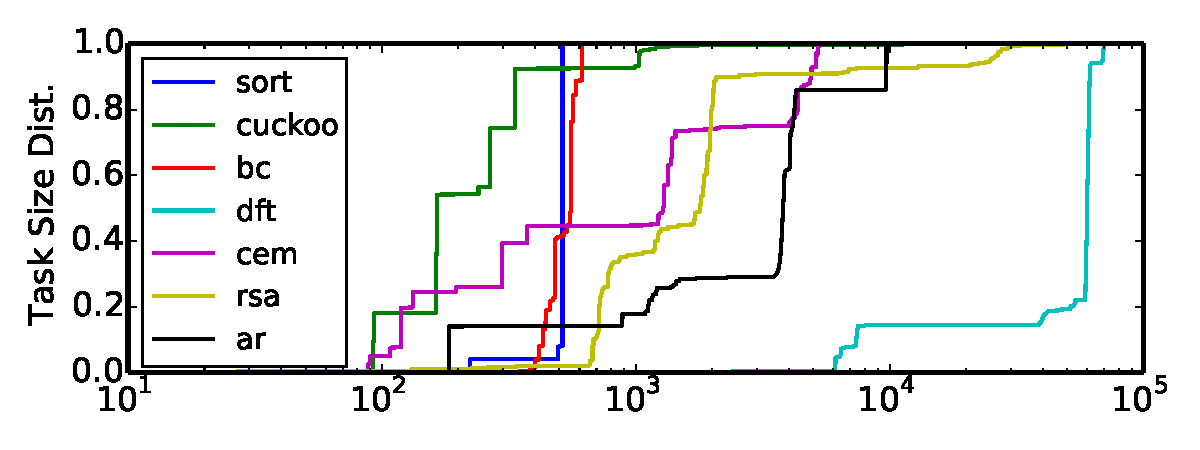
\includegraphics[width=\columnwidth]{figures/TskDist.pdf}%coalescing_timeline
	\caption{\textbf{Distribution of task sizes, estimated by task execution times.} The wide variation in task size motivates accounting for task size in the coalescing strategy.}
	\label{fig:task_profiling}
\end{figure}


%\begin{figure}
%	\centering
	%\subfloat[\sys coalesces consecutive tasks.]{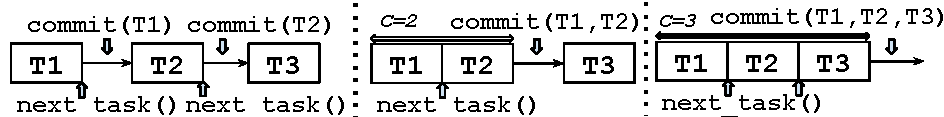
\includegraphics[width=\columnwidth]{figures/coalescing_states}\label{fig:coalescing_example_states}}\\
	%\subfloat[\sys dynamically adapts the amount of coalescing.]{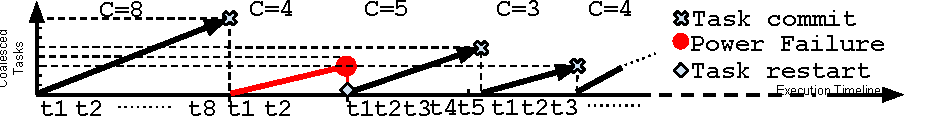
\includegraphics[width=\columnwidth]{figures/coalescing_timeline}\label{fig:coalescing_example_flowchart}}
	%\caption{\sys coalesces tasks to avoid overheads.}
	%\label{fig:coalescing_example}
%\end{figure}

%However, it takes a conservative approach by making the virtual task size equal
%to the half of the number of successfully executed real tasks before the last
%power interrupt (see lines~\ref{algo:coalescing:executionHistory1},
%\ref{algo:coalescing:executionHistory2} of Algorithm~\ref{algo:coalescing}). 
%
%We
%advocate for the algorithm conservative approach by the following two reasons:
%(i) the power interrupts are not uniformly distributed over the tasks; and (ii)
%the re-execution penalty, in case of a power interrupt, grows linearly with the
%size of a virtual task. 
%
%Furthermore, the algorithm considers the charging rate
%by allowing the real tasks counter (RTC), which represents the execution
%history between the last two power interrupts, to increase from one up to
%multiple virtual tasks (see line~\ref{algo:coalescing:realTaskCounter} of
%Algorithm~\ref{algo:coalescing}). 
%
%As a consequence, the virtual task size
%changes rapidly (since it is half of the execution history) in response to the
%change in the charging rate. 
%
%However, the algorithm sets a limit to the size of
%the virtual task for these two reasons: (i) having an infinity virtual task
%size, results in a certain computation progress loss; and (ii) the benefit of
%task merging is governed by the diminishing return principle (which will be
%demonstrated experimentally in Section~\ref{sec:results_coalescing}).
%
%The algorithm protects itself from power interrupts by going into three stages:
%(i) virtual progressing, where the operations are done on the volatile memory
%(see
%lines~\ref{algo:coalescing:virtualProgressing1}--\ref{algo:coalescing:virtualProgressing2}
%of Algorithm~\ref{algo:coalescing} ); 
%(ii) transition stage, where the volatile
%state is moved to a temporary persistent buffer. 
%
%Until the end of the second
%stage if a power is interrupted, then all the virtual progress will be
%cancelled and the virtual task will re-executed and re-initialized from a
%consistent input (see line~\ref{algo:coalescing:virtualProgressing1} of
%Algorithm~\ref{algo:coalescing}); 
%
%and (iii) persistent commit stage, upon
%entering this stage the algorithm will make a firm transition (see
%lines~\ref{algo:coalescing:firmTransition1},
%\ref{algo:coalescing:firmTransition2} of Algorithm~\ref{algo:coalescing}) and
%it will not go back to the other stages unless all the data is committed from
%the persistent buffer to non-volatile memory. 
%
%Since the data is being moved in one direction and from a persistent location,
%power interrupt is tolerable at this stage. 

%\begin{algorithm}[t]
%	\caption{\sys task coalescing mechanism}
%	\label{algo:coalescing}
%	\scriptsize
%	\begin{algorithmic}[1]
%		\State $\text{p}$  \Comment{Indicates persistent variables, initialized \textbf{only} during device programming}
%		\State $\text{RT} \in \{\sys~\text{static tasks}\}$  \Comment{Real task}
%		\State $\text{VT} \subset \{~\text{RT's}\}$  \Comment{Virtual task}
%		\State $\text{RTC}$  \Comment{RT counter}
%		\State $\text{VTC}$  \Comment{VT counter}
%		% \State $|\text{VT}|$ \Comment{VT size measured in RT}
%		\State $\text{TVT}$ \Comment{Temporary VT}
%		\State $\text{VT}_{\max}$ \Comment{Maximum VT size measured in RT (coalescing upper bound)}
%		\vspace{0.1cm}
%		
%		\State $\text{p RTC} = x $ 
%		\State $\text{p VT}_{\max} = y$
%		\State $\text{p VT} = \text{RT}$ 
%		\State $\text{p TVT} = \text{VT} $ 
%		\State $\text{VTC} = 0 $ 
%		\vspace{0.1cm}
%
%		\Function{scheduler}{\null}
%
%			\State $\text{VTC} = \text{RTC/2} $  \label{algo:coalescing:executionHistory1}
%			\State $\text{RTC} = 0 $
%			\State $\text{RT} = \text{VT}$ \Comment{Recover virtual state} \label{algo:coalescing:virtualProgressing1}
%			\If{commiting}
%				\State $\text{RT}=\text{TVT}$
%				\State $\texttt{goto} \ \ \ref{commitStage}$ \label{algo:coalescing:firmTransition1}
%			\EndIf
%			\vspace{0.1cm}
%
%			\While {True}
%				\While{$\text{VTC}--$}
%					\Function{execute}{$\text{RT}$}
%					\EndFunction
%					\If{$\text{RTC} < \text{VT}_{\max}$}
%						\State $\text{RTC}++$  \label{algo:coalescing:realTaskCounter}
%					\EndIf
%					\State $\text{RT} \leftarrow \text{RT}_{next}$ \Comment{Virtual progressing}
%				\EndWhile        \label{algo:coalescing:virtualProgressing2}
%
%				\State \Comment{Virtual task is finished}
%				\State $\text{Data} \rightarrow \text{pTempBuf}$ \Comment{pTempBuf: persistent temporary buffer}
%				\State $\text{TVT} = \text{RT}$ 
%				\State $\text{commiting} = \text{True}$ \label{algo:coalescing:firmTransition2}
%				\State 
%				\State $\text{VT} = \text{TVT}$ \label{commitStage}
%				\State $\text{pTempBuf} \rightarrow \text{FRAM}$ 
%				\State $\text{VTC} = \text{RTC/2}$ 		\Comment{Set VT size} \label{algo:coalescing:executionHistory2}
%				\State $\text{commiting} = \text{False}$ 
%
%			\EndWhile
%
%		\EndFunction
%			
%	\end{algorithmic}
%\end{algorithm}

%\subsection{Power Interrupt Immune Scheduler}
%
%% TNT :  Total Number of Tasks
% JT 	: Total Jump
% ID	: Task ID
% D	: relative Jump (Delta)
% VCT_PT : Current Task Pointer

% if(TJ < TNT)
% 	VCT_PT <- VCT_PT + D
% else
% 	while ((dis = TJ - TNT) > TNT)
% 		dis -= ID
% 	VCT_PT <- VCT_PT + dis


\begin{algorithm}[t]
	\caption{\sys's scheduler: relative jump algorithm}
	\label{algo:relativeJump}
	\scriptsize
	%\small
	\begin{algorithmic}[1]
			\State \textsf{TNT}: Total Number of Tasks
			\State \textsf{ID}: Task ID
			\State \textsf{$\delta$}: Relative Jump
			\State $\textsf{TJ} \leftarrow (\textsf{ID} + \delta )$ \Comment{Total Jump}
			\State \textsf{\textsf{$VCT_{pt}$}}: Virtual Current Task Pointer

			\If { \textsf{TJ} > \textsf{TNT} }
				\State $\textsf{dis} = \textsf{TJ} - \textsf{TNT}$
				\While{ $ \textsf{dis} > TNT $ }
					\State $\textsf{dis} -= \textsf{TNT}$
				\EndWhile
				\State $\textsf{dis} -= \textsf{ID}$
				\State \textsf{$VCT_{pt}$} $+= \textsf{dis}$
			\Else
				\State \textsf{$VCT_{pt}$} $+= \delta $

			\EndIf
	\end{algorithmic}
\end{algorithm} %Task jumping algorithm
%
%It utilizes a persistent circular buffer (i.e. persistent linked list) to keep the state of a program across power failures. \sys provides an API to enable a programmer to have a full control over the execution flow of the program, i.e. (un)blocking a task or re-execute the same task which is particularly important in the intermittent execution to emulate a persistent loop. \todo{Expand this section}{Amjad}
%
%\begin{algorithm}
%	\caption{Opportunistic virtual Task size}
%	\label{algo:fixVirtTask}
%	\scriptsize
%	%\small
%	\begin{algorithmic}[1]
%		\State $VT \subset \text{\{\sys Tasks\}} $  \Comment{$VT:$ Virtual Task}
%		\State VTS : VT size
%		\vspace{0.1cm}
%		
%		\While {$True$}
%		\State $VT \leftarrow VT_{next}$
%		\vspace{0.1cm}
%		\While {execute $VT$} 
%		\If { $\text{power failed twice}$ }				
%		\State $VTS--$  
%		\EndIf
%		\EndWhile
%		
%		\vspace{0.1cm}
%		\If {$ \text{All tasks executed}$}
%		\State $VTS++$
%		\EndIf
%		\EndWhile
%	\end{algorithmic}
%\end{algorithm}
